\begin{frame}{Case Studies}
\begin{columns}
  \column{0.48\linewidth}
  \begin{outline}
    \1 Three Case Studies
    \2 PIN-protected backup
    \2 Password hashing
    \2 TOTP Token
    \1 Source on \href{https://github.com/anishathalye/knox-hsm}{Github}
  \end{outline}

  \column{0.48\linewidth}
  \centering
  \begin{center}
  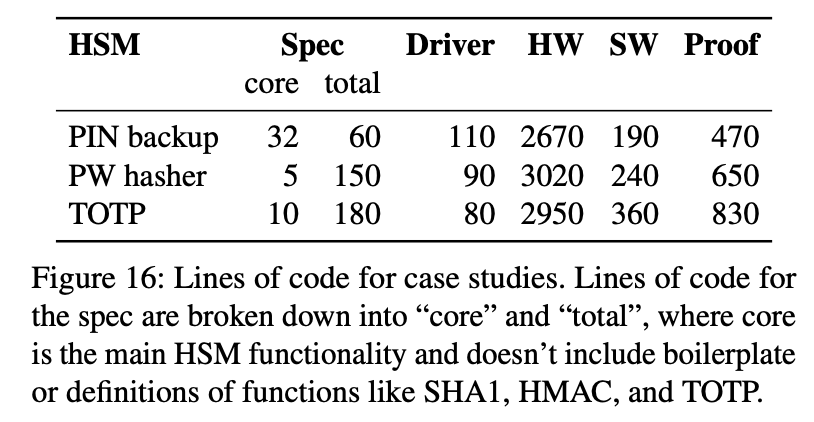
\includegraphics[width=4cm]{fig_16.png}

  \vspace{0.5cm}

  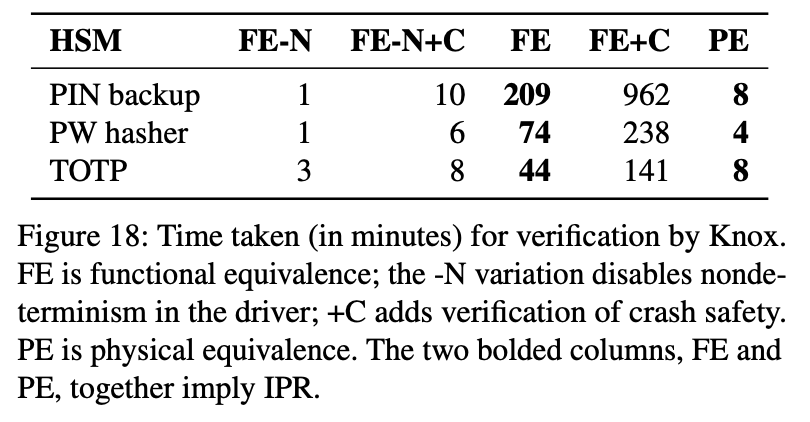
\includegraphics[width=4cm]{fig_18.png}
\end{center}
\end{columns}
\end{frame}

\begin{frame}{Case Study: PIN-protected backup HSM}
\begin{columns}
  \column{0.48\linewidth}
  \begin{outline}
    \1 Runs on RISC-V CPU
    \1 Features
    \2 Multiple Secrets
    \2 Enforce Attempts Limit
    \1 Emulator Implementation
    \2 Constructive
    \2 Inject spec output into circuit
    \1 Bugs Found
    \2 Timing attack with \lstinline{strcmp}
    \2 Guess timing attack 
  \end{outline}
  \column{0.48\linewidth}
  \centering
  \begin{center}
    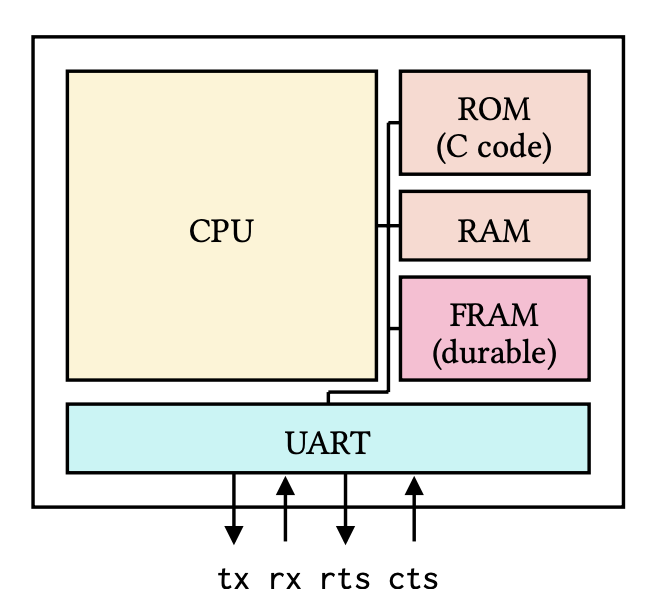
\includegraphics[width=4cm]{ppb_ex_diagram.png}
  \end{center}
\end{columns}
\end{frame}

\begin{frame}{Case Study: Password Hashing HSM}
\begin{columns}
  \column{0.48\linewidth}
  \begin{outline}
    \1 Includes \lstinline{sha256}
    \2 Needs spec
    \2 Verilog implementation
    \1 Can't retrieve secret
    \1 Crash Safe 
    \2 Multiword writes
    \2 Caught timing bug
    \1 Caught \lstinline{mem_addr} bug
  \end{outline}

  \column{0.48\linewidth}
  \centering
  \begin{center}
  \shadowimage[width=5cm]{ppb_ex_spec.png}
\end{center}
\end{columns}
\end{frame}

\placelogofalse
\begin{frame}{Case Study: TOTP Token}
\begin{columns}
  \column{0.48\linewidth}
  \begin{outline}
    \1 Host provides timestamp
    \1 Can't rewind timestamp
    \1 Includes \lstinline{SHA1} 
    \1 Issue with symbolic execution
    \1 Timing attack with \lstinline{\%} 
  \end{outline}

  \column{0.48\linewidth}
  \centering
  \begin{center}
  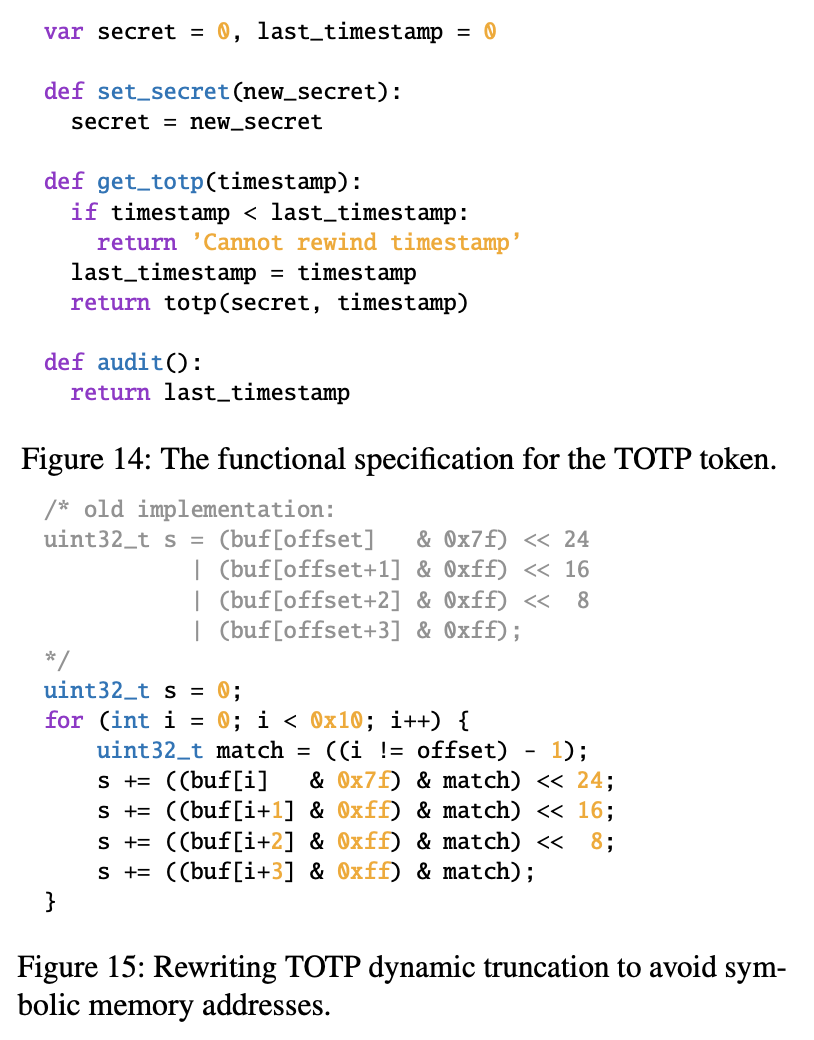
\includegraphics[width=5cm]{totp_spec.png}
  \end{center}
\end{columns}
\end{frame}
\placelogotrue
